%%
%% Copyright (c) 2018-2019 Weitian LI <liweitianux@sjtu.edu.cn>
%% Creative Commons BY 4.0
%%

\chapter{射电晕对宇宙再电离探测的影响}
\label{chap:halo}

%=====================================================================
\section{评估方法}
\label{sec:eval-method}

利用\autoref{chap:simulation}模拟得到的射电晕、EoR 信号以及其他前景成分的
SKA1-Low 观测图像,我们可以定量地评估射电晕将对 EoR 探测产生的影响.
我们将分别针对\ac{fg-rm}和\ac{fg-avd}两类前景处理方法 (\autoref{sec:fg-methods})
进行评估.
首先,我们计算一维\ac{ps}来对比射电晕和 EoR 信号在各个尺度 $k$ 的总体功率,
说明使用\ac{fg-rm}方法时将面临的射电晕的污染强度.
其次,我们计算二维\ac{ps},然后在 EoR 窗口 (\autoref{sec:eor-window})
内比较射电晕和 EoR 信号的功率,
据此评估射电晕的污染将会对使用\ac{fg-avd}方法产生多大程度的影响.

\begin{figure}[htp]
  \centering
  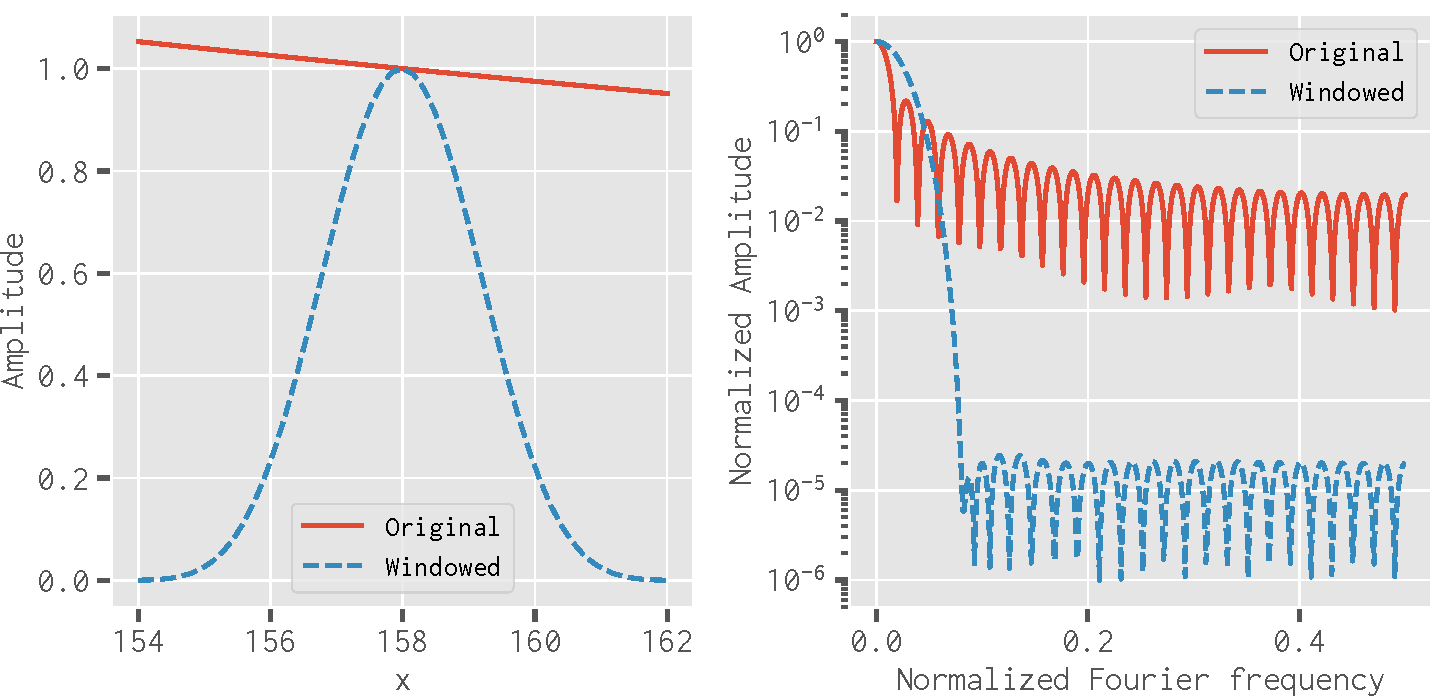
\includegraphics[width=\textwidth]{ft-sidelobes}
  \bicaption[加窗前后的 Fourier 变换结果对比]{%
    直接进行 Fourier 变换(红色实线)与
    使用 Blackman--Nuttall \acs*{f-window}之后再 Fourier 变换(蓝色虚线)
    的结果对比.
    左栏显示了加窗前后的输入信号 $y = (x/158)^{-2}$,
    右栏显示了相应的 Fourier 变换结果.
  }{%
    A comparison of the Fourier transform results with and without
    applying the Blackman--Nuttall window function.
    The left panel shows the original input signal $y = (x/158)^{-2}$
    (solid red line) and the windowed signal (dashed blue line);
    the right panel shows the corresponding Fourier transform results.
  }
  \label{fig:ft-sidelobes}
\end{figure}

考虑一个有限宽的频带,信号(如前景辐射)将在频带的两端出现跃变,
这种边界效应会导致 Fourier 变换的结果具有显著的\ac{sidelobe}.
即使输入信号非常平滑,Fourier 变换后也会出现一系列幅度较大的高频 Fourier 成分,
如\autoref{fig:ft-sidelobes} 所示.
为了抑制边界效应所产生的\ac{sidelobe},可以先对信号加窗,然后再进行 Fourier 变换.
一个常用的选择是 Blackman--Nuttall \ac{f-window},
该\ac{f-window}具有良好的\ac{sidelobe}性质 \cite{nuttall1981}:
\begin{equation}
  \label{eq:bn-window}
  w[n] = a_0 - a_1 \cos\left(\frac{2\Cpi n}{N}\right)
    + a_2 \cos\left(\frac{4\Cpi n}{N}\right)
    - a_3 \cos\left(\frac{6\Cpi n}{N}\right) ,
\end{equation}
其中
$N$ 为采样点的数目(即窗的宽度),
其他系数分别为:
$a_0 = \num{0.3635819}$,
$a_1 = \num{0.4891775}$,
$a_2 = \num{0.1365995}$,
$a_3 = \num{0.0106411}$.
\autoref{fig:ft-sidelobes} 显示了使用 Blackman--Nuttall \ac{f-window}
之后得到的 Fourier 变换结果,可见高频 Fourier 成分的幅度被有效地抑制了.
因此,我们对\autoref{chap:simulation}模拟得到的\ac{imgcube}沿频率方向施加
Blackman--Nuttall \ac{f-window}然后再计算\ac{ps}
\cite{trott2015,chapman2016}.


%=====================================================================
\section{一维功率谱}
\label{sec:ps1d}

\begin{figure}[htp]
  \centering
  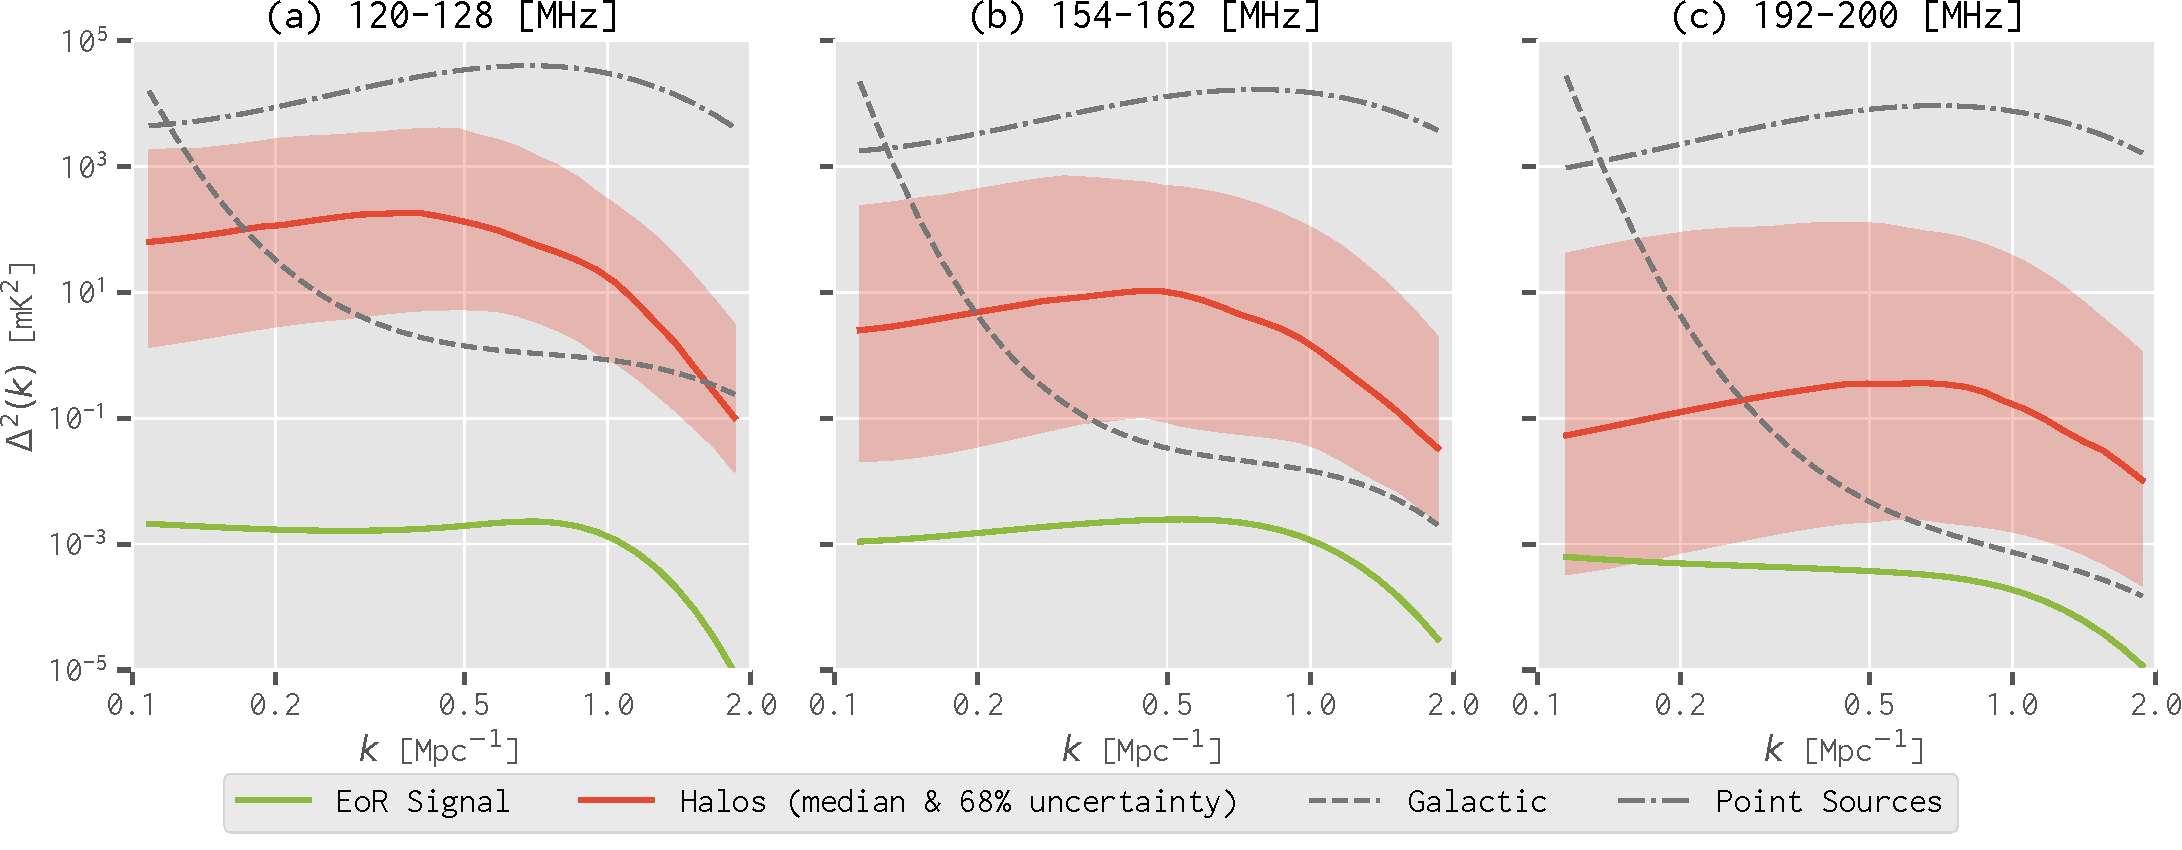
\includegraphics[width=\textwidth]{ps1d-3bands}
  \bicaption[各成分在三个频带内的一维功率谱 $\ac{psD}(k)$ 对比]{%
    EoR 信号(绿色实线)、射电晕(红色实线)、银河系弥散辐射(灰色虚线)以及
    河外点源(灰色点虚线)之间的一维功率谱 $\ac{psD}(k)$ 的对比.
    左栏、中栏、右栏分别表示 \numrange{120}{128}、\numrange{154}{162}
    和 \numrange{192}{200} \si{\MHz} 三个频带的结果.
    对于射电晕,红色实线及其阴影区域分别表示从 100 次模拟结果中得到的
    中位数和 68\% 的误差范围.
  }{%
    Comparisons of the 1D dimensionless power spectra $\ac{psD}(k)$
    among the EoR signal (solid green line), radio halos (solid red line),
    Galactic diffuse emission (dashed gray line), and extragalactic point
    sources (dash-dotted gray line) in the
    \textbf{(a)} \SIrange{120}{128}{\MHz},
    \textbf{(b)} \SIrange{154}{162}{\MHz}, and
    \textbf{(c)} \SIrange{192}{200}{\MHz} frequency bands.
    The solid red lines and shaded regions represent the median values
    and the corresponding 68\% uncertainties of the power
    spectra for radio halos estimated from the 100 simulation runs.
  }
  \label{fig:ps1d-3bands}
\end{figure}

我们对上一章模拟得到的每一个成分在每一个频带里的\ac{imgcube}分别计算了
一维\ac{ps} $\ac{psD}(k)$.
对于射电晕,我们使用了全部 100 次模拟 (\autoref{sec:halo-maps}) 的结果
来估算其一维功率谱的中位数和 68\% 的误差范围.
具体而言,在一个频带里,射电晕的 100 次模拟会生成 100 个\ac{imgcube},
分别计算这 100 个\ac{imgcube}的一维功率谱,
然后从所得的 100 个一维功率谱计算每个尺度 $k$ 处的中位数和相应的 68\% 误差范围.
\autoref{fig:ps1d-3bands} 显示了各成分在三个频带内的
一维功率谱 $\ac{psD}(k)$ 的对比.
可见,在 $\SI{0.1}{\per\Mpc} < k < \SI{2}{\per\Mpc}$ 尺度上,
射电晕的典型功率(红色实线)在 \numrange{120}{128}、\numrange{154}{162} 和
\numrange{192}{200} \si{\MHz} 频带内分别是 EoR 信号的功率的
\num{e4}、\num{e3} 和 \num{e2.5} 倍.
考虑到不同天区内射电晕的亮度和数目的显著涨落,
在 68\% 的误差范围内(红色阴影区域),
射电晕的功率能够变化约 \numrange{10}{100} 倍.

对于另外两个前景成分,银河系前景在最大尺度 ($k \lesssim \SI{0.1}{\per\Mpc}$)
上是最强的污染源,但随着尺度 $k$ 的减小,其功率也迅速减小.
在 $\SI{0.5}{\per\Mpc} \lesssim k \lesssim \SI{1}{\per\Mpc}$
的中小尺度范围,
射电晕的典型功率将是银河系前景的功率的约 \numrange{10}{100} 倍.
河外点源除了在最大尺度上弱于银河系前景,在其他尺度上均是最强的污染源.

以上这些结果清楚地说明射电晕是严重的 EoR 前景污染源,需要在前景扣除中被仔细处理.
此外,射电晕还具有一定的形态结构,显著增加了对其准确建模和扣除的难度.


%=====================================================================
\section{二维功率谱}
\label{sec:ps2d}

\begin{figure}[htp]
  \centering
  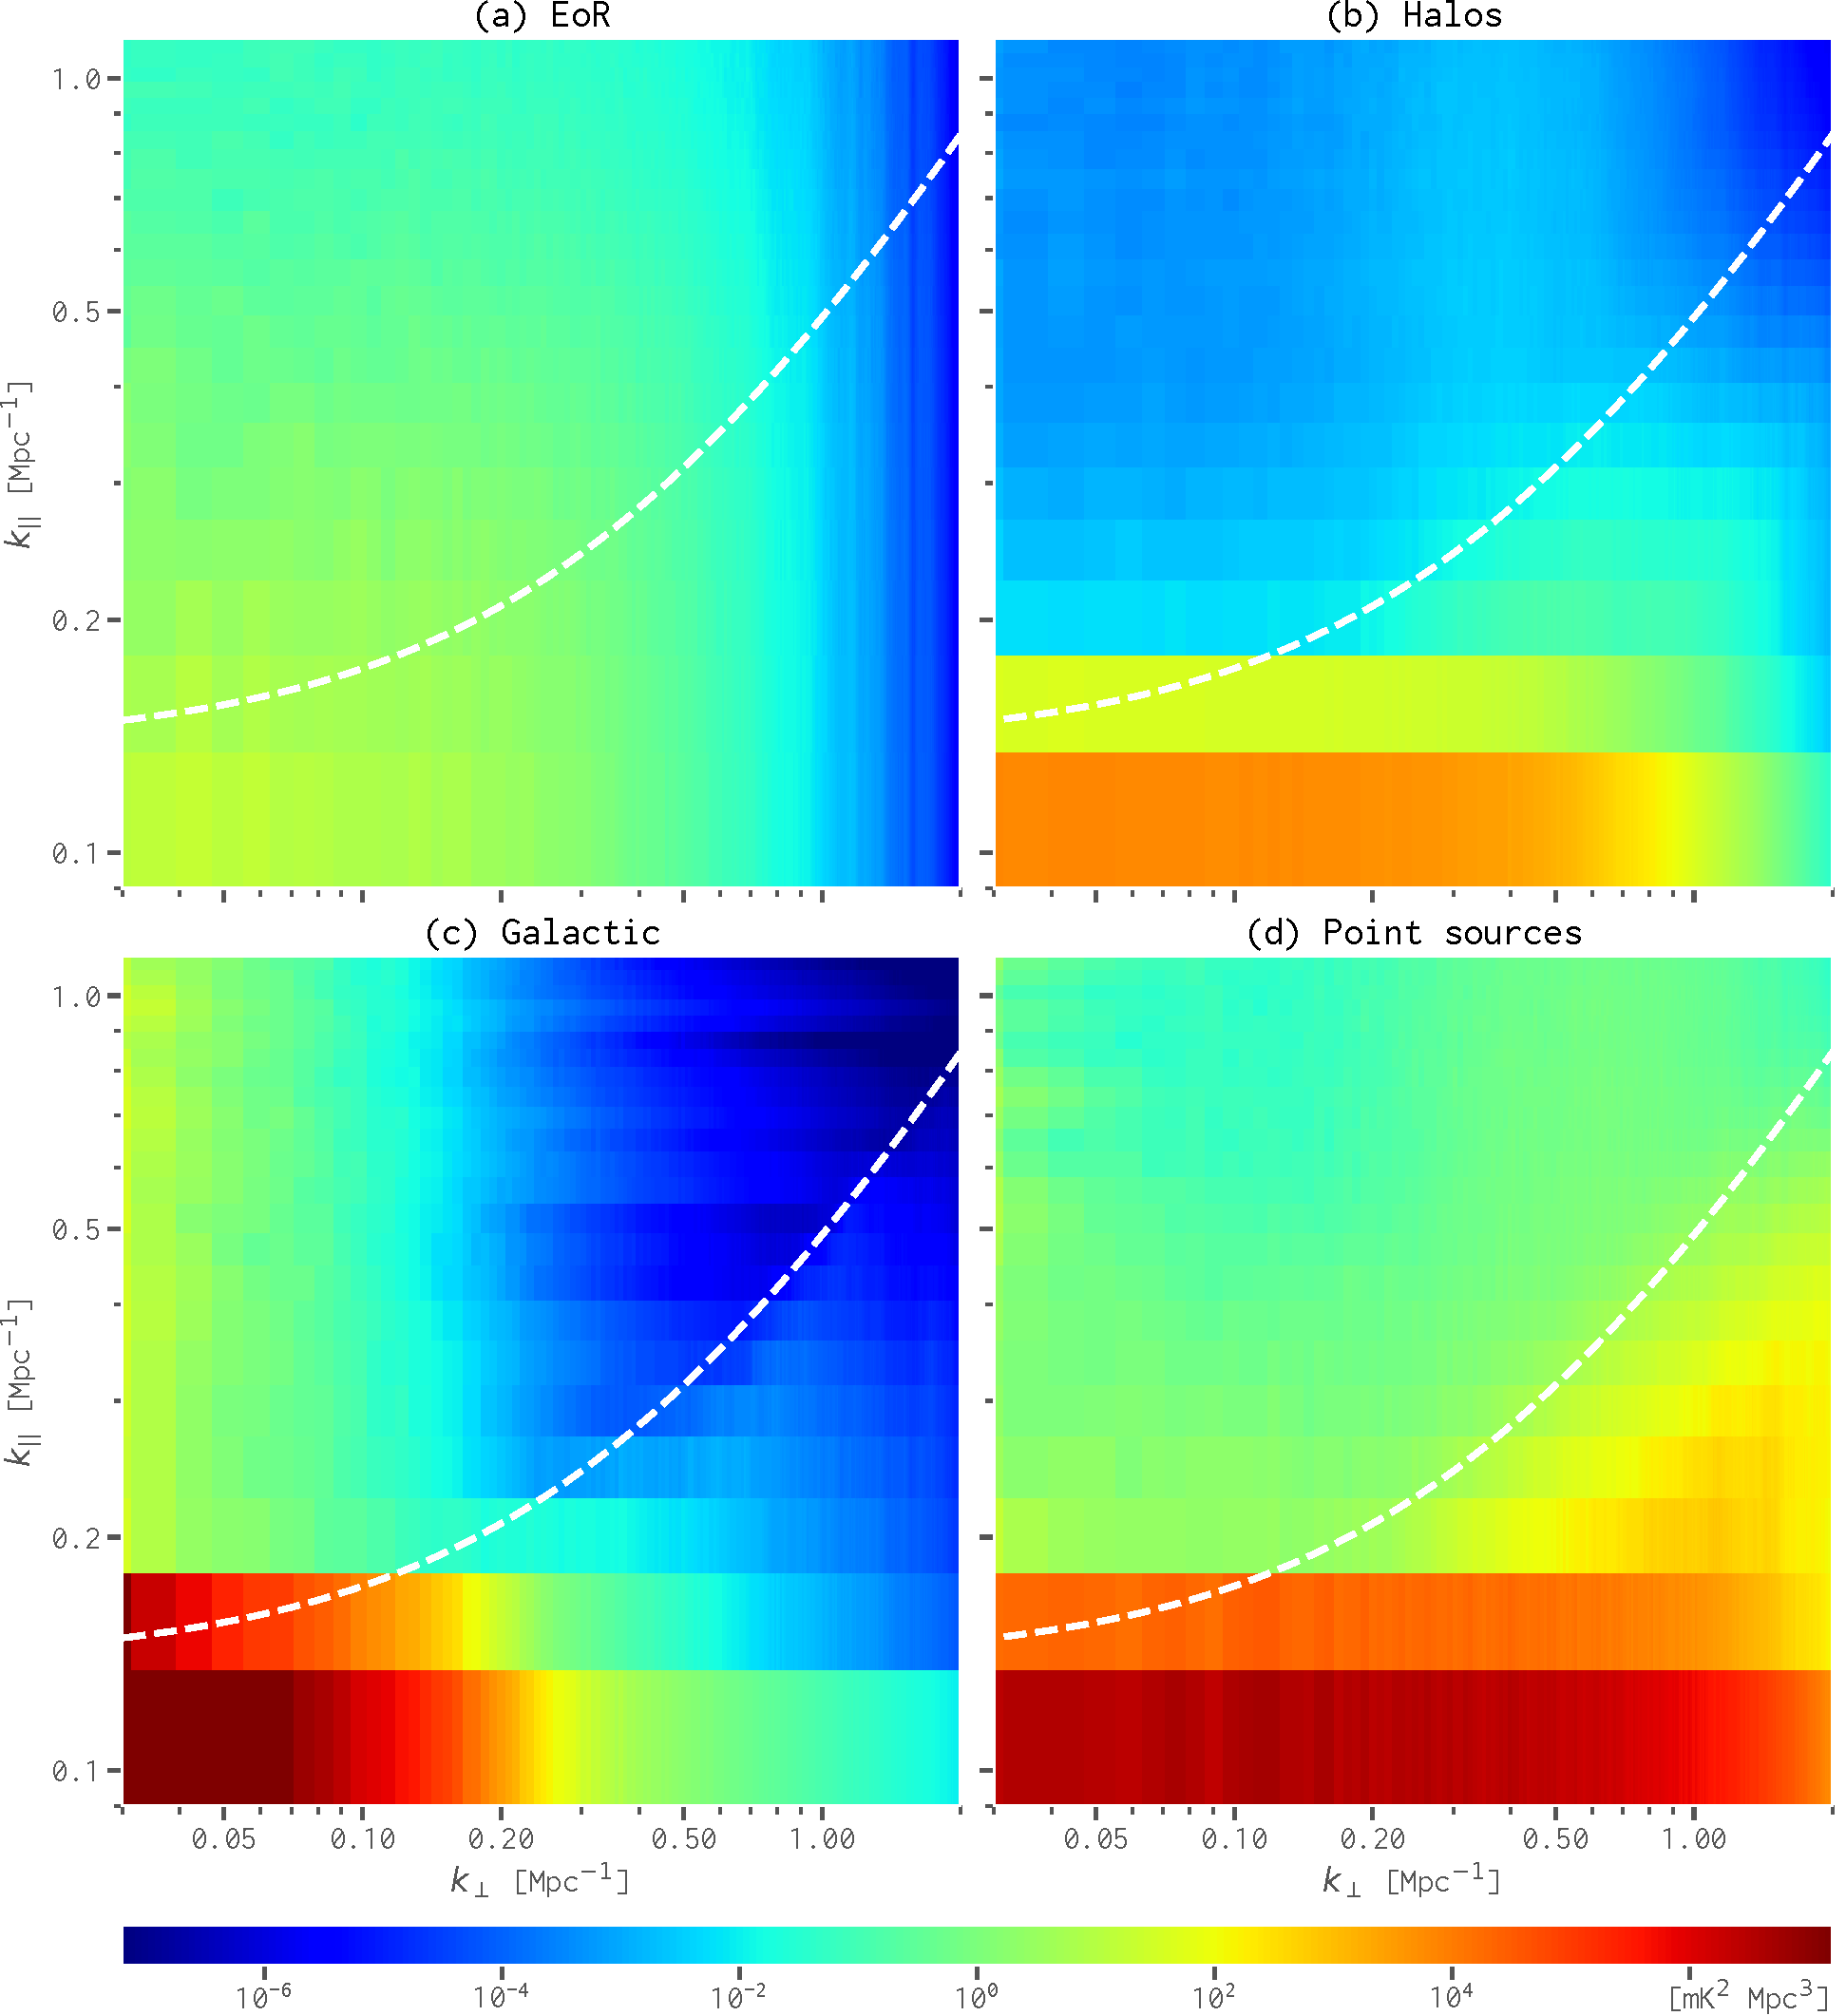
\includegraphics[width=\textwidth]{ps2d-band158}
  \bicaption[%
    各成分在 \SIrange{154}{162}{\MHz} 频段的二维功率谱
    $\ac{psD}(\kperp, \klos)$%
  ]{%
    各成分在 \SIrange{154}{162}{\MHz} 频段的二维功率谱
    $\ac{psD}(\kperp, \klos)$,
    从左上至右下分别为:
    \textbf{(a)} EoR 信号;
    \textbf{(b)} 射电晕(100 次模拟的中位数);
    \textbf{(c)} 银河系弥散辐射;
    \textbf{(d)} 河外点源.
    所有子图共用了以 [\si{\mK\squared\Mpc\cubed}] 为单位的对数\ac{colorbar}.
    图中的白色虚线显示了 EoR 窗口的边界.
  }{%
    The \SIrange{154}{162}{\MHz} 2D power spectra
    $\ac{psD}(\kperp, \klos)$ of
    \textbf{(a)} the EoR signal,
    \textbf{(b)} radio halos (median of the 100 simulation runs),
    \textbf{(c)} Galactic diffuse emission,
    and
    \textbf{(d)} extragalactic point sources.
    All panels share the same logarithmic scale in units of
    [\si{\mK\squared\Mpc\cubed}].
    The dashed white lines mark the boundary between the EoR window
    (at the top left) and the contaminating wedge (at the bottom right).
  }
  \label{fig:ps2d}
\end{figure}

以 \SIrange{154}{162}{\MHz} 频带为例,
\autoref{fig:ps2d} 显示了 EoR 信号、射电晕、银河系弥散辐射以及河外点源的
二维功率谱 $\ac{psD}(\kperp, \klos)$,
其中射电晕的二维功率谱对应于 100 次模拟结果的中位数.
从图中容易看出,EoR 信号的功率分散在大范围的 \klos{} \ac{mode}里,
反映了 EoR 信号沿频率维度快速变化的特点;
频谱光滑的前景成分则集中在 \klos{} 较小的区域
($\klos \lesssim \SI{0.2}{\per\Mpc}$).
在空间维度 \kperp{},射电晕的功率主要出现在
$\kperp \lesssim \SI{1}{\per\Mpc}$ 的范围,
并且倾向于集中在 $\kperp \sim \SI{0.5}{\per\Mpc}$ 的中等尺度上.
同时,银河系弥散辐射的功率主导了 $\kperp \lesssim \SI{0.1}{\per\Mpc}$
的大尺度区域,而河外点源的功率则占据了 $\kperp \gtrsim \SI{0.1}{\per\Mpc}$
的中小尺度范围.
这些结果与 \autoref{fig:ps1d-3bands}(b) 所展示的结果是相符的,
还与诸多文献中的结果是一致的 \cite{datta2010,trott2015,barry2016,chapman2016}.

\begin{figure}[htp]
  \centering
  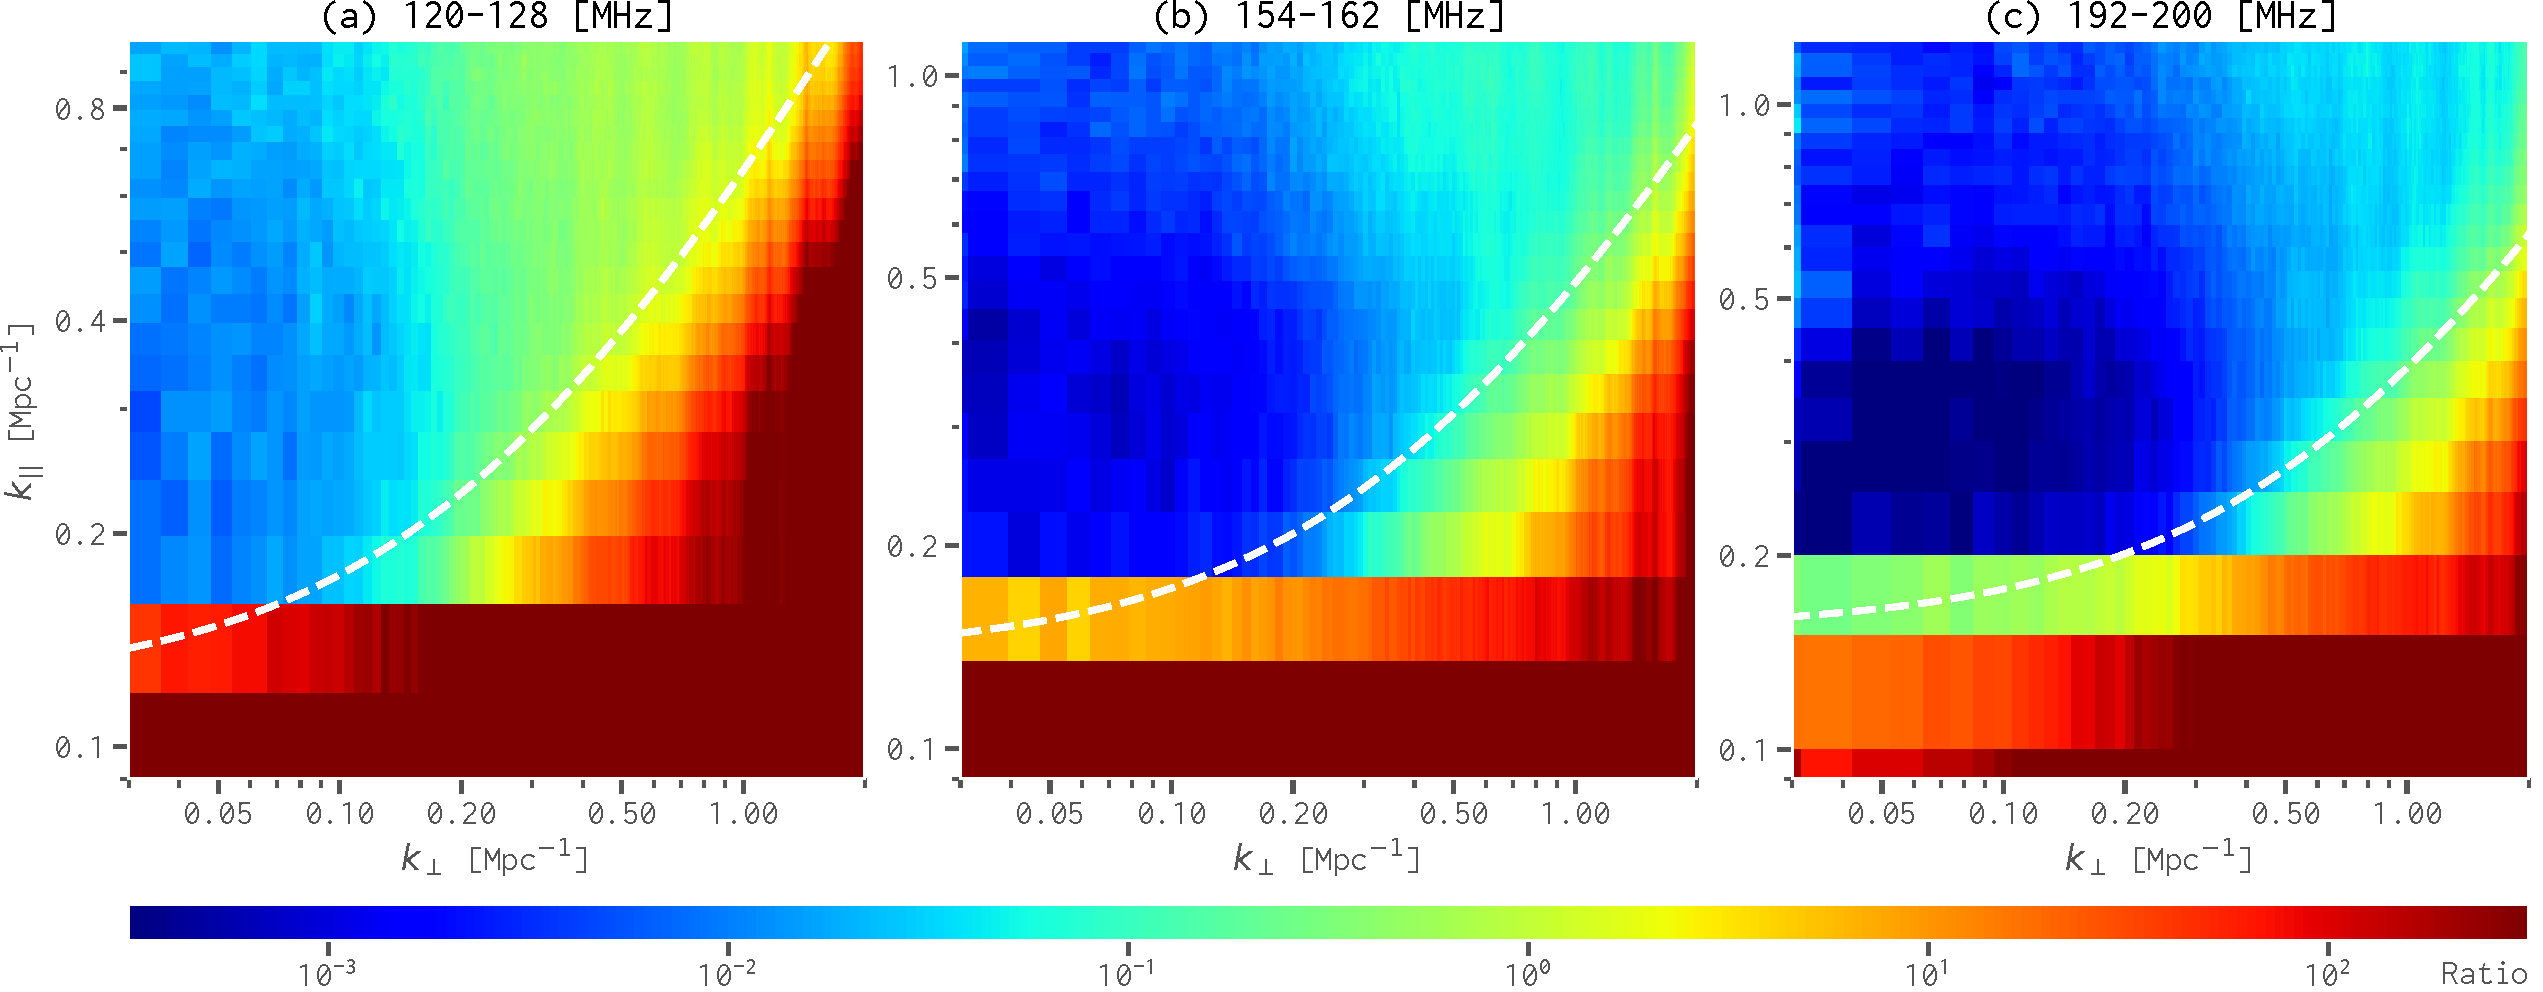
\includegraphics[width=\textwidth]{ps2d-ratio-3bands}
  \bicaption[射电晕和 EoR 信号的二维功率比 $R(\kperp, \klos)$]{%
    射电晕和 EoR 信号在
    \textbf{(a)} \SIrange{120}{128}{\MHz}、
    \textbf{(b)} \SIrange{154}{162}{\MHz} 和
    \textbf{(c)} \SIrange{192}{200}{\MHz}
    三个频带内的二维功率比 $R(\kperp, \klos)$.
    这里使用的射电晕二维功率谱对应于 100 次模拟结果的中位数.
    所有子图共用了对数\ac{colorbar}.
    图中的白色虚线显示了 EoR 窗口的边界.
  }{%
    The 2D power spectrum ratios $R(\kperp, \klos)$ of radio halos to the
    EoR signal in the
    \textbf{(a)} \SIrange{120}{128}{\MHz},
    \textbf{(b)} \SIrange{154}{162}{\MHz}, and
    \textbf{(c)} \SIrange{192}{200}{\MHz} frequency bands.
    The median 2D power spectrum of 100 simulation runs for radio halos
    is used.
    All panels use the same color bar in logarithmic scale.
    The dashed white lines mark the EoR window boundaries.
  }
  \label{fig:ps2d-ratio}
\end{figure}

为了更具体地显示射电晕对 EoR 信号的污染情况,
我们将射电晕的二维功率谱 $\Delta^2_{\R{halo}}(\kperp, \klos)$
除以 EoR 信号的二维功率谱 $\Delta^2_{\R{eor}}(\kperp, \klos)$,
得到两者的二维功率比:
\begin{equation}
  R(\kperp, \klos)
    \equiv \frac{\Delta^2_{\R{halo}}(\kperp, \klos)}{
      \Delta^2_{\R{eor}}(\kperp, \klos)} .
\end{equation}
如\autoref{fig:ps2d-ratio} 所示,
可见射电晕的污染区域形成一个明显的楔形 (\autoref{sec:eor-window}).
我们发现,在 \SIrange{120}{128}{\MHz} 频带内,
射电晕在 $\kperp \gtrsim \SI{0.1}{\per\Mpc}$ 的尺度范围内
对 EoR 信号产生了严重污染(两者功率比值 $R \gtrsim 1$).
在 \numrange{154}{162} 和 \numrange{192}{200} \si{\MHz} 两个频带里,
射电晕的主要污染范围分别为 $\kperp \gtrsim \SI{0.3}{\per\Mpc}$
和 $\kperp \gtrsim \SI{0.5}{\per\Mpc}$.
同时容易看出,射电晕在较低频率处 ($\sim$\,\SI{120}{\MHz})
对 EoR 测量的污染程度明显比在较高频率处 ($\sim$\,\SI{200}{\MHz})
的污染程度要强.
\autoref{fig:ps1d-3bands} 也显示了与此一致的结果.

\begin{figure}[htp]
  \centering
  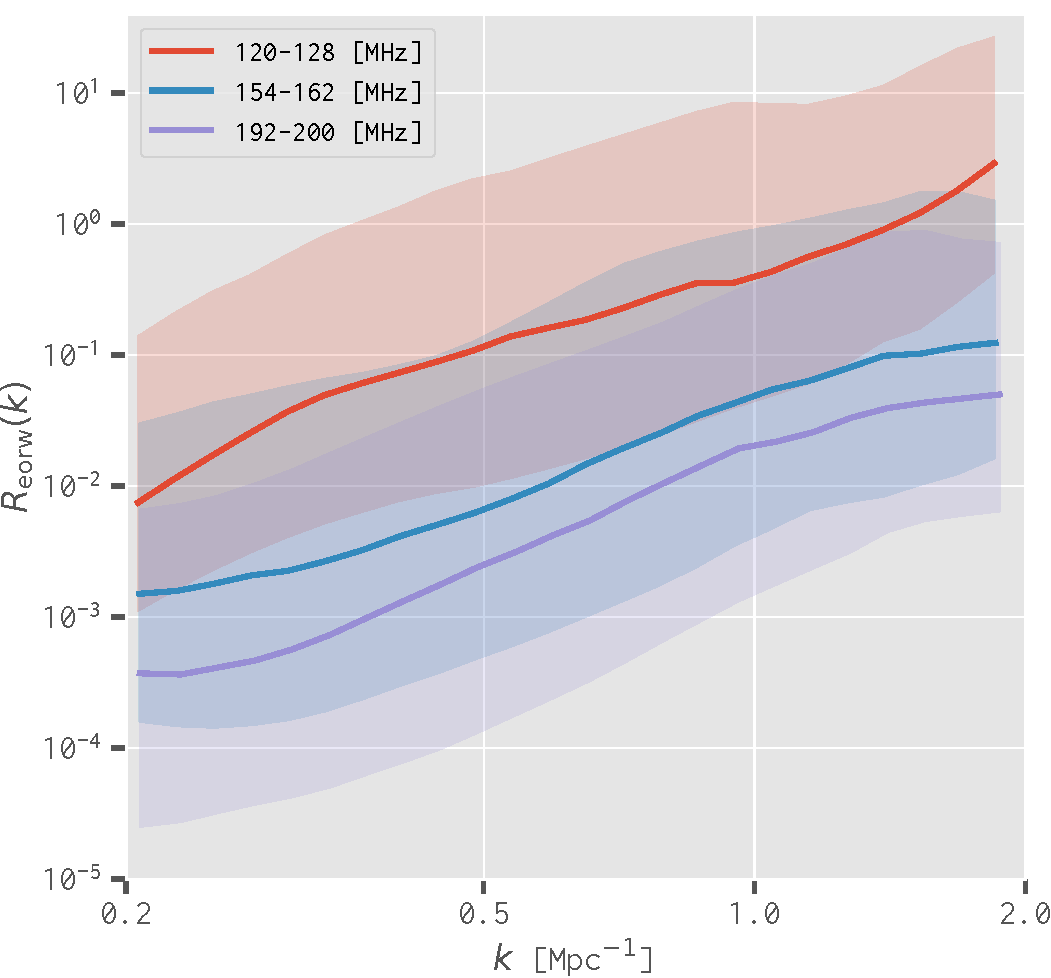
\includegraphics[width=0.8\textwidth]{ps1d-ratio-3bands}
  \bicaption[射电晕和 EoR 信号在 EoR 窗口内的一维功率比 $R_{\R{eorw}}(k)$]{%
    射电晕和 EoR 信号在 EoR 窗口内的一维功率比 $R_{\R{eorw}}(k)$.
    实线和阴影区域分别对应于射电晕 100 次模拟结果的中位数和 68\% 误差范围.
  }{%
    The 1D power ratios $R_{\R{eorw}}(k)$ inside the EoR window of
    radio halos to the EoR signal.
    The solid lines and shaded regions show the median values and
    corresponding 68\% uncertainties, respectively.
  }
  \label{fig:ps1d-ratio}
\end{figure}

考虑到射电晕的污染主要集中在二维功率谱右下方的楔形区域内
(如\autoref{fig:ps2d-ratio} 所示),
因此可以选定一个合适的边界将其排除,
于是便可以在左上方的 EoR 窗口内提取 EoR 信号,
有效地避开了强烈的前景污染,这就是\ac{fg-avd}方法的基本思路.
利用\autoref{eq:eor-window} 定义的 EoR 窗口边界的表达式,
我们测试了多种不同的 ($w$, $\Phi$) 参数组合,
最终选择了 $w = 3$ 以及 $\Phi = 1.5\,\ac{Fov}$,
即 $\Phi$ 在 \numrange{120}{128}、\numrange{154}{162}
和 \numrange{192}{200} \si{\MHz} 三个频带的值分别为
$\Phi_{124} = \SI{7.5}{\degree}$、
$\Phi_{158} = \SI{6.0}{\degree}$ 和
$\Phi_{196} = \SI{4.8}{\degree}$.
\autoref{fig:ps2d} 和\autoref{fig:ps2d-ratio} 显示了如此定义的 EoR 窗口边界,
可见能够很好地避开\ac{fg-wedge}的污染.
但是,在 \numrange{120}{128}、\numrange{154}{162}
和 \numrange{192}{200} \si{\MHz} 三个频带内,
EoR 信号分别有约 55\%、54\% 和 40\% 的功率损失在避开的\ac{fg-wedge}之中.

在以上定义的 EoR 窗口内,对射电晕和 EoR 信号的二维功率比 $R(\kperp, \klos)$ 平均,
得到一维功率比 $R_{\R{eorw}}(k)$,如\autoref{fig:ps1d-ratio} 所示.
相比\autoref{fig:ps1d-3bands} 所示的未受 EoR 窗口约束的一维功率谱 $\ac{psD}(k)$,
射电晕的污染在 EoR 窗口内被抑制了约 4 个数量级.
比如,在 $k \sim \SI{1}{\per\Mpc}$ 尺度上,
EoR 窗口内的一维功率比 $R_{\R{eorw}}(k)$ 在 \numrange{120}{128}、
\numrange{154}{162} 和 \numrange{192}{200} \si{\MHz}
三个频带的典型值(图中的实线)分别约为 45\%、6\% 和 2\%.
这充分展示了 EoR 窗口和\ac{fg-avd}法是探测 EoR 信号的有力工具.
尽管如此,由于射电晕的亮度和数目在不同天区里具有显著的涨落,
在 68\% 的误差范围(图中的阴影区域)以及
$\SI{0.5}{\per\Mpc} \lesssim k \lesssim \SI{1}{\per\Mpc}$ 尺度范围内,
EoR 窗口内的一维功率比 $R_{\R{eorw}}(k)$ 在三个频带内的值能够分别达到约
\numrange{230}{800}\%、\numrange{18}{95}\% 和 \numrange{7}{40}\%,
说明射电晕泄漏到 EoR 窗口内的功率仍然可能是显著的,
尤其是在较低频率 ($\sim$\,\SI{120}{\MHz}).

基于本节和上一节 (\autoref{sec:ps1d}) 的结果,
我们认为射电晕是 EoR 信号探测的一个重要前景干扰成分.
即使在一个已避开严重污染的 EoR 窗口内,射电晕所产生的污染仍然能够
对 EoR 信号的准确测量产生不可忽略的干扰,尤其是在 $\sim$\,\SI{120}{\MHz} 的较低频率.
为了获得一个尽可能干净、同时也尽可能大的 EoR 窗口,
深入理解、建模并扣除射电晕以及其他前景干扰成分是非常必要的,
还需要联合使用\ac{fg-rm}和\ac{fg-avd}两类方法,改进 EoR 信号探测手段.


%=====================================================================
\section{频谱伪结构的影响}
\label{sec:freq-artifacts}

\autoref{sec:obs-simu} 模拟了理想情况下的射电干涉观测,
但是,实际观测所面临的情况要复杂得多,
比如,仪器的校准存在不确定性、电离层的扰动、复杂的数据处理;
参见 \autoref{sec:det-difficulties}.
这些复杂的仪器效应和观测效应会导致\ac{imgcube}的频谱出现伪结构,
破坏前景辐射的频谱光谱性,从而阻碍 EoR 信号的有效分离.

一些模拟和观测研究指出,干涉阵列的频率\ac{channel}的校准存在约
\numrange{0.1}{1}\% 的不确定性
\cite{barry2016,beardsley2016,ewallWice2017}.
我们对\ac{imgcube}的每一个\ac{slice}乘以一个服从平均值为 0、
标准差为 σ 的正态分布的随机数,
以此模拟实际观测中出现的频谱伪结构 \cite{chapman2016};
然后计算有无频谱伪结构的\ac{imgcube}的\ac{ps}并进行对比,
从而评估频谱伪结构对\ac{ps}以及前景干扰的影响.
我们考虑如下两种边界情况:
\begin{itemize}
  \item 频谱伪结构的幅度为 $A_{\R{arti}} = 0.1\%$,
    对应于正态分布的标准差为 $σ = 0.001$;
  \item 频谱伪结构的幅度为 $A_{\R{arti}} = 1\%$,对应于 $σ = 0.01$.
\end{itemize}

\begin{figure}[htp]
  \centering
  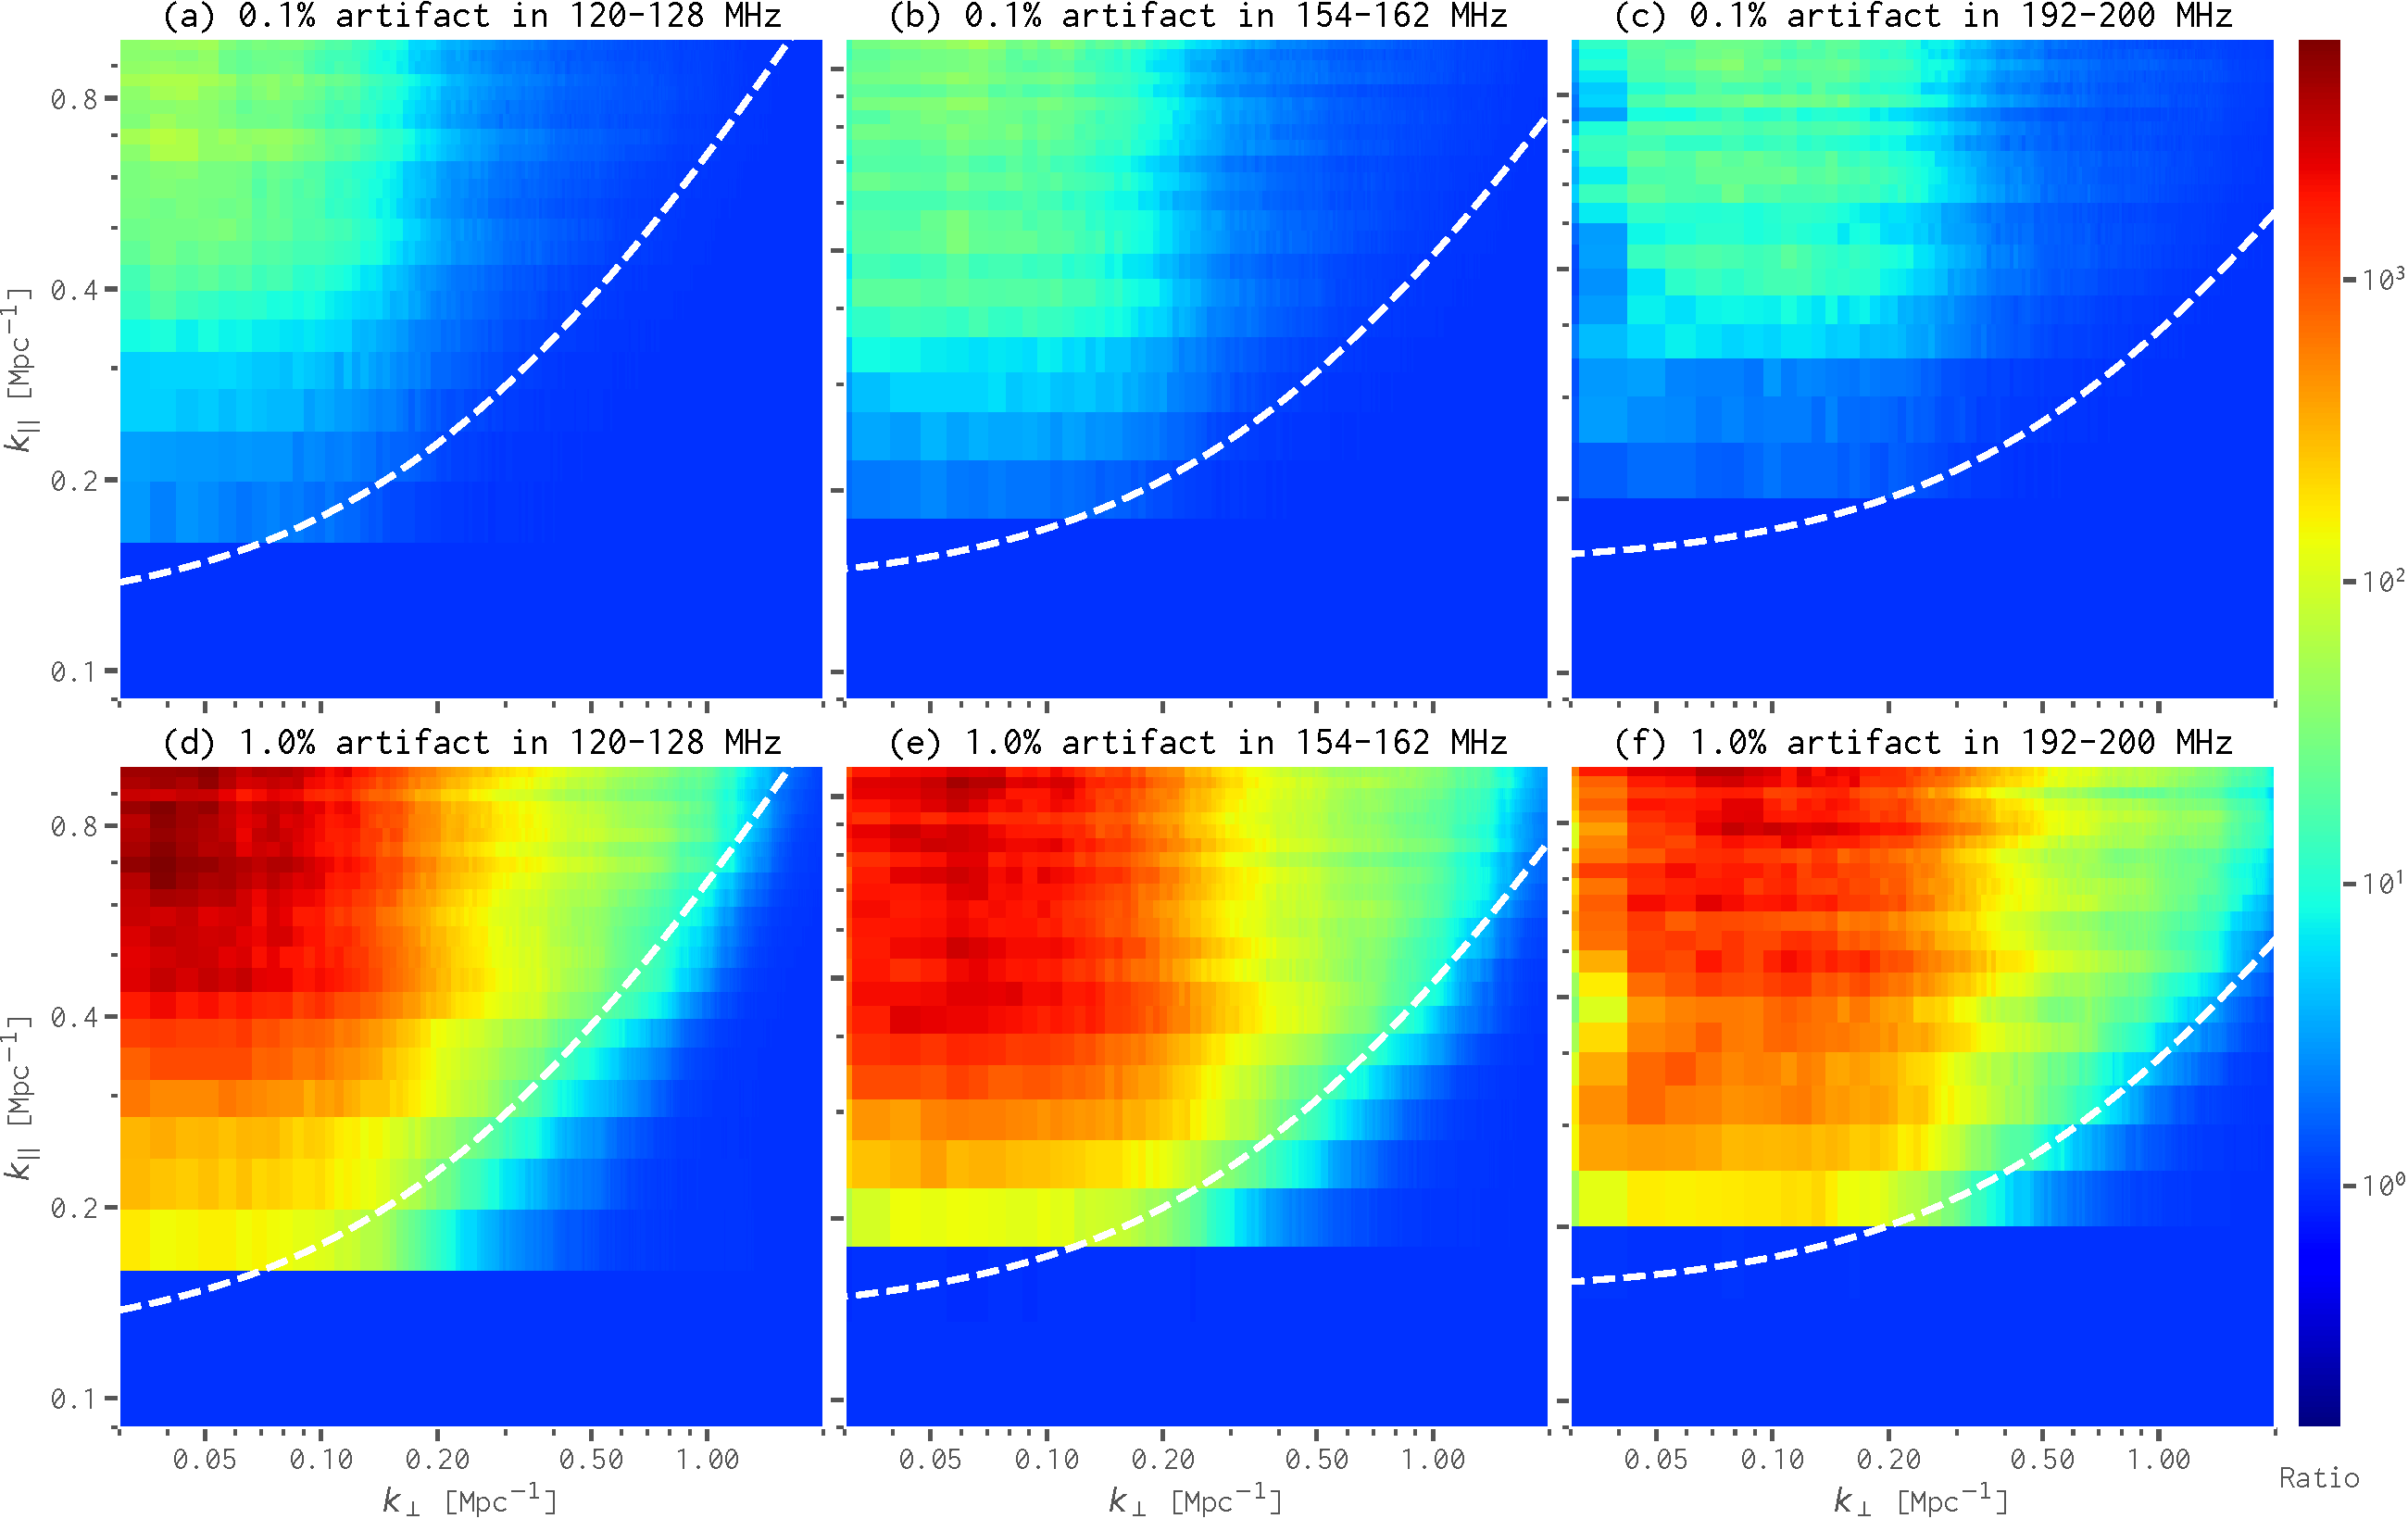
\includegraphics[width=0.75\textwidth]{ps2d-ratio-crp-3bands}
  \bicaption[有无频谱伪结构时射电晕的二维功率比 $R_{\R{arti}}(\kperp, \klos)$]{%
    有无频谱伪结构时射电晕的二维功率比 $R_{\R{arti}}(\kperp, \klos)$.
    上、中、下三行分别对应 \numrange{120}{128}、\numrange{154}{162} 和
    \numrange{192}{200} \si{\MHz} 三个频带;
    左、右两列分别显示了频谱伪结构幅度为 $A_{\R{arti}} = 0.1\%$
    和 $A_{\R{arti}} = 1\%$ 的情况;
    白色虚线标识了 EoR 窗口的边界.
    所有子图共用了对数\ac{colorbar}.
  }{%
    The 2D power spectrum ratios $R_{\R{arti}}(\kperp, \klos)$
    of radio halos with and without frequency artifacts.
    The upper, middle, and lower rows show the power spectrum ratios
    in the \numrange{120}{128}, \numrange{154}{162}, and
    \numrange{192}{200} \si{\MHz} bands, respectively;
    the left and right columns show the cases of frequency artifacts
    being $A_{\R{arti}} = 0.1\%$ and $A_{\R{arti}} = 1\%$, respectively.
    The dashed white lines mark the EoR window boundaries.
    All panels share the same color bar in logarithmic scale.
  }
  \label{fig:ps2d-ratio-crp}
\end{figure}

给定一个\ac{imgcube},我们计算在有频谱伪结构和无频谱伪结构情形下的二维功率谱,
分别为 $\Delta^2_{\R{arti}}(\kperp, \klos)$ 和 $\Delta^2(\kperp, \klos)$,
于是可得两者之比为:
\begin{equation}
  R_{\R{arti}}(\kperp, \klos)
    \equiv \frac{\Delta^2_{\R{arti}}(\kperp, \klos)}{
      \Delta^2(\kperp, \klos)} .
\end{equation}
对于射电晕的 100 次模拟,我们计算了每一次模拟在 \numrange{120}{128}、
\numrange{154}{162} 和 \numrange{192}{200} \si{\MHz} 三个频带内、
频谱伪结构幅度为 $A_{\R{arti}} = 0.1\%$ 和 $A_{\R{arti}} = 1\%$
的情形下的二维功率比 $R_{\R{arti}}(\kperp, \klos)$,
据此得到射电晕在三个频带内以及两种频谱伪结构幅度的情况下的二维功率比的中位数,
结果如\autoref{fig:ps2d-ratio-crp} 所示.
我们发现,频谱伪结构使射电晕的二维功率谱受到了严重破坏.
在 $\kperp \lesssim \SI{0.2}{\per\Mpc}$ 和
$\klos \gtrsim \SI{0.3}{\per\Mpc}$ 尺度范围内,
幅度为 $A_{\R{arti}} = 0.1\%$ 的频谱伪结构使射电晕在 \numrange{120}{128}、
\numrange{154}{162} 和 \numrange{192}{200} \si{\MHz}
三个频带内的功率分别增加了约 17、15 和 13 倍.
当频谱伪结构的幅度为 $A_{\R{arti}} = 1\%$,即为前一种情况的 10 倍时,
射电晕在相同尺度范围内的功率则为前一种情况的 100 倍,
即在三个频带内的功率比 $R$ 分别约为 1700、1500 和 1300.

作为对比,我们对 EoR 信号的\ac{imgcube}引入了同样的频谱伪结构
($A_{\R{arti}} = 0.1\%$ 或 $1\%$)
并计算了相应的二维功率比 $R_{\R{arti}}(\kperp, \klos)$.
但是,我们发现 EoR 信号的二维功率谱几乎未受到频谱伪结构的影响,
即使频谱伪结构的幅度为 $A_{\R{arti}} = 1\%$.
这主要是因为 EoR 信号在频率维度已经具有明显的小尺度起伏结构.

因此,即使是非常微小(幅度约为 $\sim$\,0.1\%)的频谱伪结构
也会使射电晕的干扰显著增强,特别是在关键的 EoR 窗口内.
这说明 EoR 探测实验需要对仪器进行非常严格的校准,
以获得非常准确的频谱响应 \cite{barry2016}.
同时,这些结果也进一步支持我们在 \autoref{sec:ps2d} 所得的结论:
射电晕对 EoR 探测而言是一个严重的前景干扰成分.


%=====================================================================
\section{远旁瓣的影响}
\label{sec:fscn}

低频干涉阵列的波束形状非常复杂,除\ac{mainlobe}外还有一系列明显的\ac{sidelobe}
\cite{noordam2004,wijnholds2010},
如\autoref{fig:ska-beams} 显示了 SKA1-Low 在 100 和 200 MHz 处模拟的站点波束.
更多关于 SKA1-Low 的波束形状及其旁瓣的性质可见 \citeay{mort2017}.
辐射源即使远离\ac{mainlobe},也会通过\ac{sidelobe}在视场中产生类似噪声的干扰,
这就是\emph{\acf{fscn}} \cite{smirnov2012}.
更加重要的是,当观测的 $uv$ 覆盖达到饱和时,\ac{fscn} 便不再降低,
因此,\ac{fscn} 可能会强于仪器的热噪声而成为制约成像质量的关键因素 \cite{mort2017}.

\begin{figure}[htp]
  \centering
  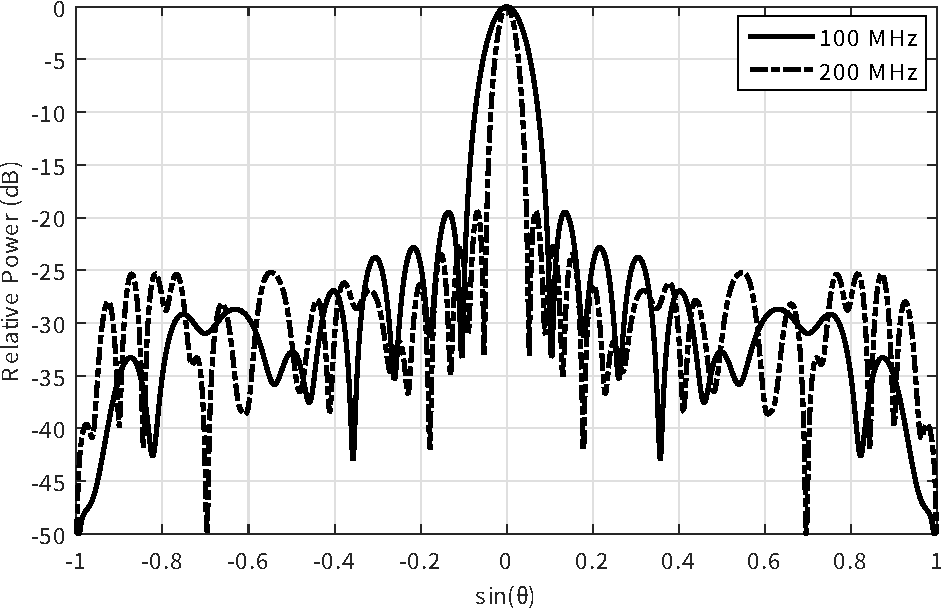
\includegraphics[width=\textwidth]{SKA1-low-beams}
  \bicaption[模拟的 SKA1-Low 站点波束]{%
    在 100 和 200 MHz 处模拟的 SKA1-Low 站点波束.
  }{%
    The simulated station beams of SKA1-Low at 100 and 200 MHz.
    \\来源/Credit:
    \citeay{mort2017}. [删减了标识]
  }
  \label{fig:ska-beams}
\end{figure}

为了研究位于\ac{sidelobe}中的射电晕所产生的 \ac{fscn},
我们需要生成相应的天图,然后输入 \texttt{OSKAR} 软件开展模拟观测.
\texttt{OSKAR} 利用了射电干涉仪测量方程 (measurement equation) \cite{smirnov2011},
实现了逼真的\ac{bf},并且能够开展全天模拟 \cite{mort2010}.
我们取 \SIrange{154}{162}{\MHz} 频带为例,
首先模拟射电晕的天图,其中射电晕覆盖了从第二\ac{sidelobe}的边缘
(距离视场中心 $\phi \sim \SI{10}{\degree}$)
一直到地平线 ($\phi = \SI{90}{\degree}$) 的范围.
这相当于在实际数据处理中将\ac{mainlobe}和第一\ac{sidelobe}里的射电晕
全部识别并完全去除.
然后,使用 \texttt{OSKAR} 和 \texttt{WSClean} 软件按
\autoref{sec:obs-simu} 所述方法进行模拟观测并成像,
得到视场中央 \SI{5 x 5}{\degree} 区域的\ac{dirty-map}.
对频带内的所有频率\ac{channel}均如此处理,
于是得到射电晕 \ac{fscn} 的\ac{imgcube},
最后计算其二维功率谱 $\Delta^2_{\R{fscn}}(\kperp, \klos)$.

\begin{figure}[htp]
  \centering
  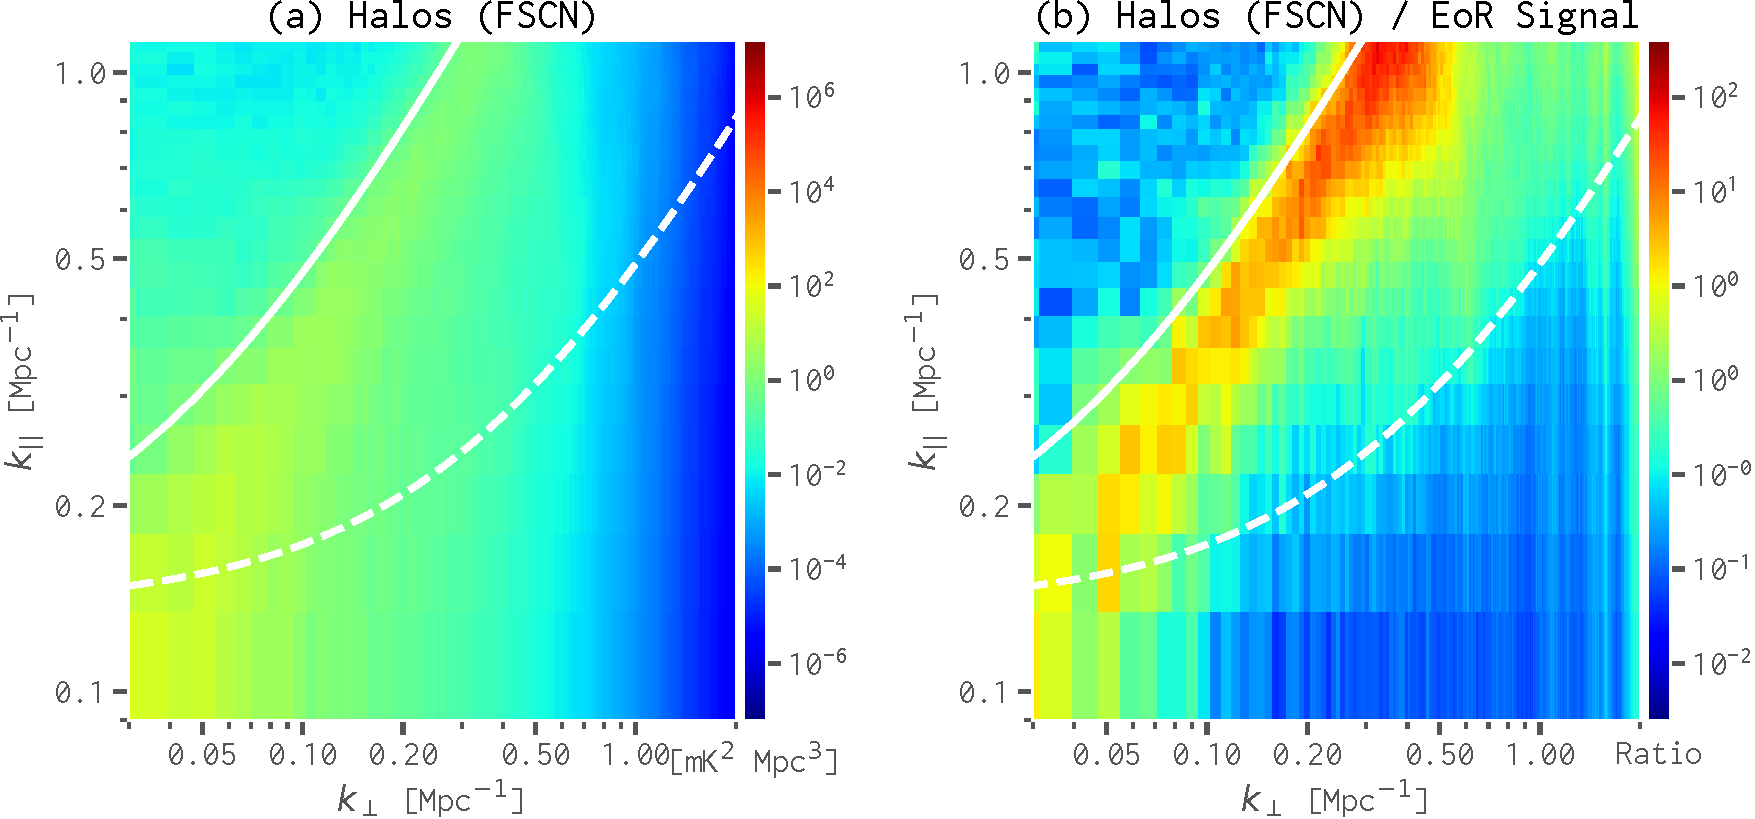
\includegraphics[width=\textwidth]{ps2d-fscn}
  \bicaption[射电晕 FSCN 的二维功率谱及其与 EoR 信号的功率谱对比]{%
    \emph{(a)} 射电晕 FSCN 的二维功率谱 $\Delta^2_{\R{fscn}}(\kperp, \klos)$;
    \emph{(b)} 射电晕 FSCN 与 EoR 信号的二维功率比 $R_{\R{fscn}}(\kperp, \klos)$.
    白色虚线和实线分别标识了 $\Phi = \SI{6}{\degree}$ 和 \SI{90}{\degree}
    所对应的 EoR 窗口边界.
  }{%
    \emph{(a)} The 2D power spectrum of the FSCN caused by radio halos
    in the far side-lobes of the station beam.
    \emph{(b)} The 2D power spectrum ratio of the FSCN to the EoR signal.
    The results are derived in the \SIrange{154}{162}{\MHz} band.
    The dashed and solid white lines mark the EoR window boundaries
    defined with $\Phi = \SI{6}{\degree}$ and \SI{90}{\degree},
    respectively.
  }
  \label{fig:ps2d-fscn}
\end{figure}

\autoref{fig:ps2d-fscn} 显示了射电晕 \ac{fscn}
的二维功率谱 $\Delta^2_{\R{fscn}}(\kperp, \klos)$
以及与 EoR 信号的二维功率比 $R_{\R{fscn}}(\kperp, \klos)$.
我们发现,射电晕 \ac{fscn} 将对 EoR 信号产生的干扰;
在 $\kperp \sim \SI{0.3}{\per\Mpc}$ 和 $\klos \sim \SI{1.0}{\per\Mpc}$
的尺度范围内,射电晕 \ac{fscn} 的功率达到了 EoR 信号的约 20 倍.
显然可见,\ac{fg-wedge}污染区域跨过原来的边界(白色虚线)向左上方增长了很多,
极大地压缩了 EoR 窗口的大小.
为了能够有效地避开 \ac{fscn} 的污染,我们被迫采用一个更加保守的 EoR 窗口边界,
如图中白色实线所示的、由 $\Phi = \SI{90}{\degree}$ 确定的边界,
但是将损失绝大部分的 EoR 信号.

因此,严重的 \ac{fscn} 污染使得筛选 EoR 观测天区成为一个更加困难的任务,
因为不仅在\ac{mainlobe}里,还有在\ac{sidelobe}里,
原则上都不允许存在明亮的射电晕以及其他干扰源.
否则需要在一个远远大于视场的天区里,准确识别、建模并扣除这些干扰源,
如此将显著增加数据处理的难度 \cite{pober2013,pober2016}.


%=====================================================================
\section{小结}

Based on the Press--Schechter formalism and merger-induced turbulent
re-acceleration model, we have simulated the emission maps of radio halos,
for which we have incorporated the SKA1-Low's instrumental effects by
utilizing its latest layout configuration.
By carrying out detailed comparisons of power spectra between radio halos
and the EoR signal as well as the Galactic diffuse emission and
extragalactic point sources in the \numrange{120}{128},
\numrange{154}{162}, and \numrange{192}{200} \si{\MHz} bands,
we have shown that radio halos are severe contaminating sources,
especially toward lower frequencies ($\sim$\,\SI{120}{\MHz}).
Even if inside the properly defined EoR windows, radio halos can still
be non-negligible contaminating sources to EoR observations.
Moreover, we have investigated the contamination resulted from
frequency artifacts and radio halos located inside the far side-lobes,
both of which support our conclusion that radio halos are severe
foreground contaminating sources and need careful treatments in the
forthcoming deep EoR observations.

本章内容已发表于 \apj{} (ApJ) \cite{li.halo}.


%% EOF
